\chapter{Electronics Essentials}
Electronics is a facinating world. This beginner's guide will introduce you to the essential
components and tools you'll need to start building your own simple circuits. We'll cover the
basics of breadboards, LEDs, buttons, resistors, and jumper cables. You should feel free to
explore on your own as well using the components in your kit. While this guide will be useful,
it is not even close to everything you'll need to know. There is always more to learn and if
electronics interests you, there are lots of online tutorials as well as formal education to
guide you further.

\section{The Breadboard: Your Circuit's Foundation}
\subsection{What is a breadboard?}

A breadboard is a reusable platform for prototyping electronic circuits without the need for
soldering. It's a plastic board with numerous tiny holes arranged in rows and columns. These holes
are connected internally, making it easy to connect components together.

\subsection{Understanding the layout}
\subsubsection{Power rails}
The long horizontal rows along the top and bottom edges are typically used as power rails to
distribute power (positive and negative) throughout the circuit.
\subsubsection{Internal connections}
The remaining rows are divided into vertical columns, with each column having five holes connected
internally. These connections allow you to easily connect multiple components within the same column.

\begin{figure}[H]
\centering
    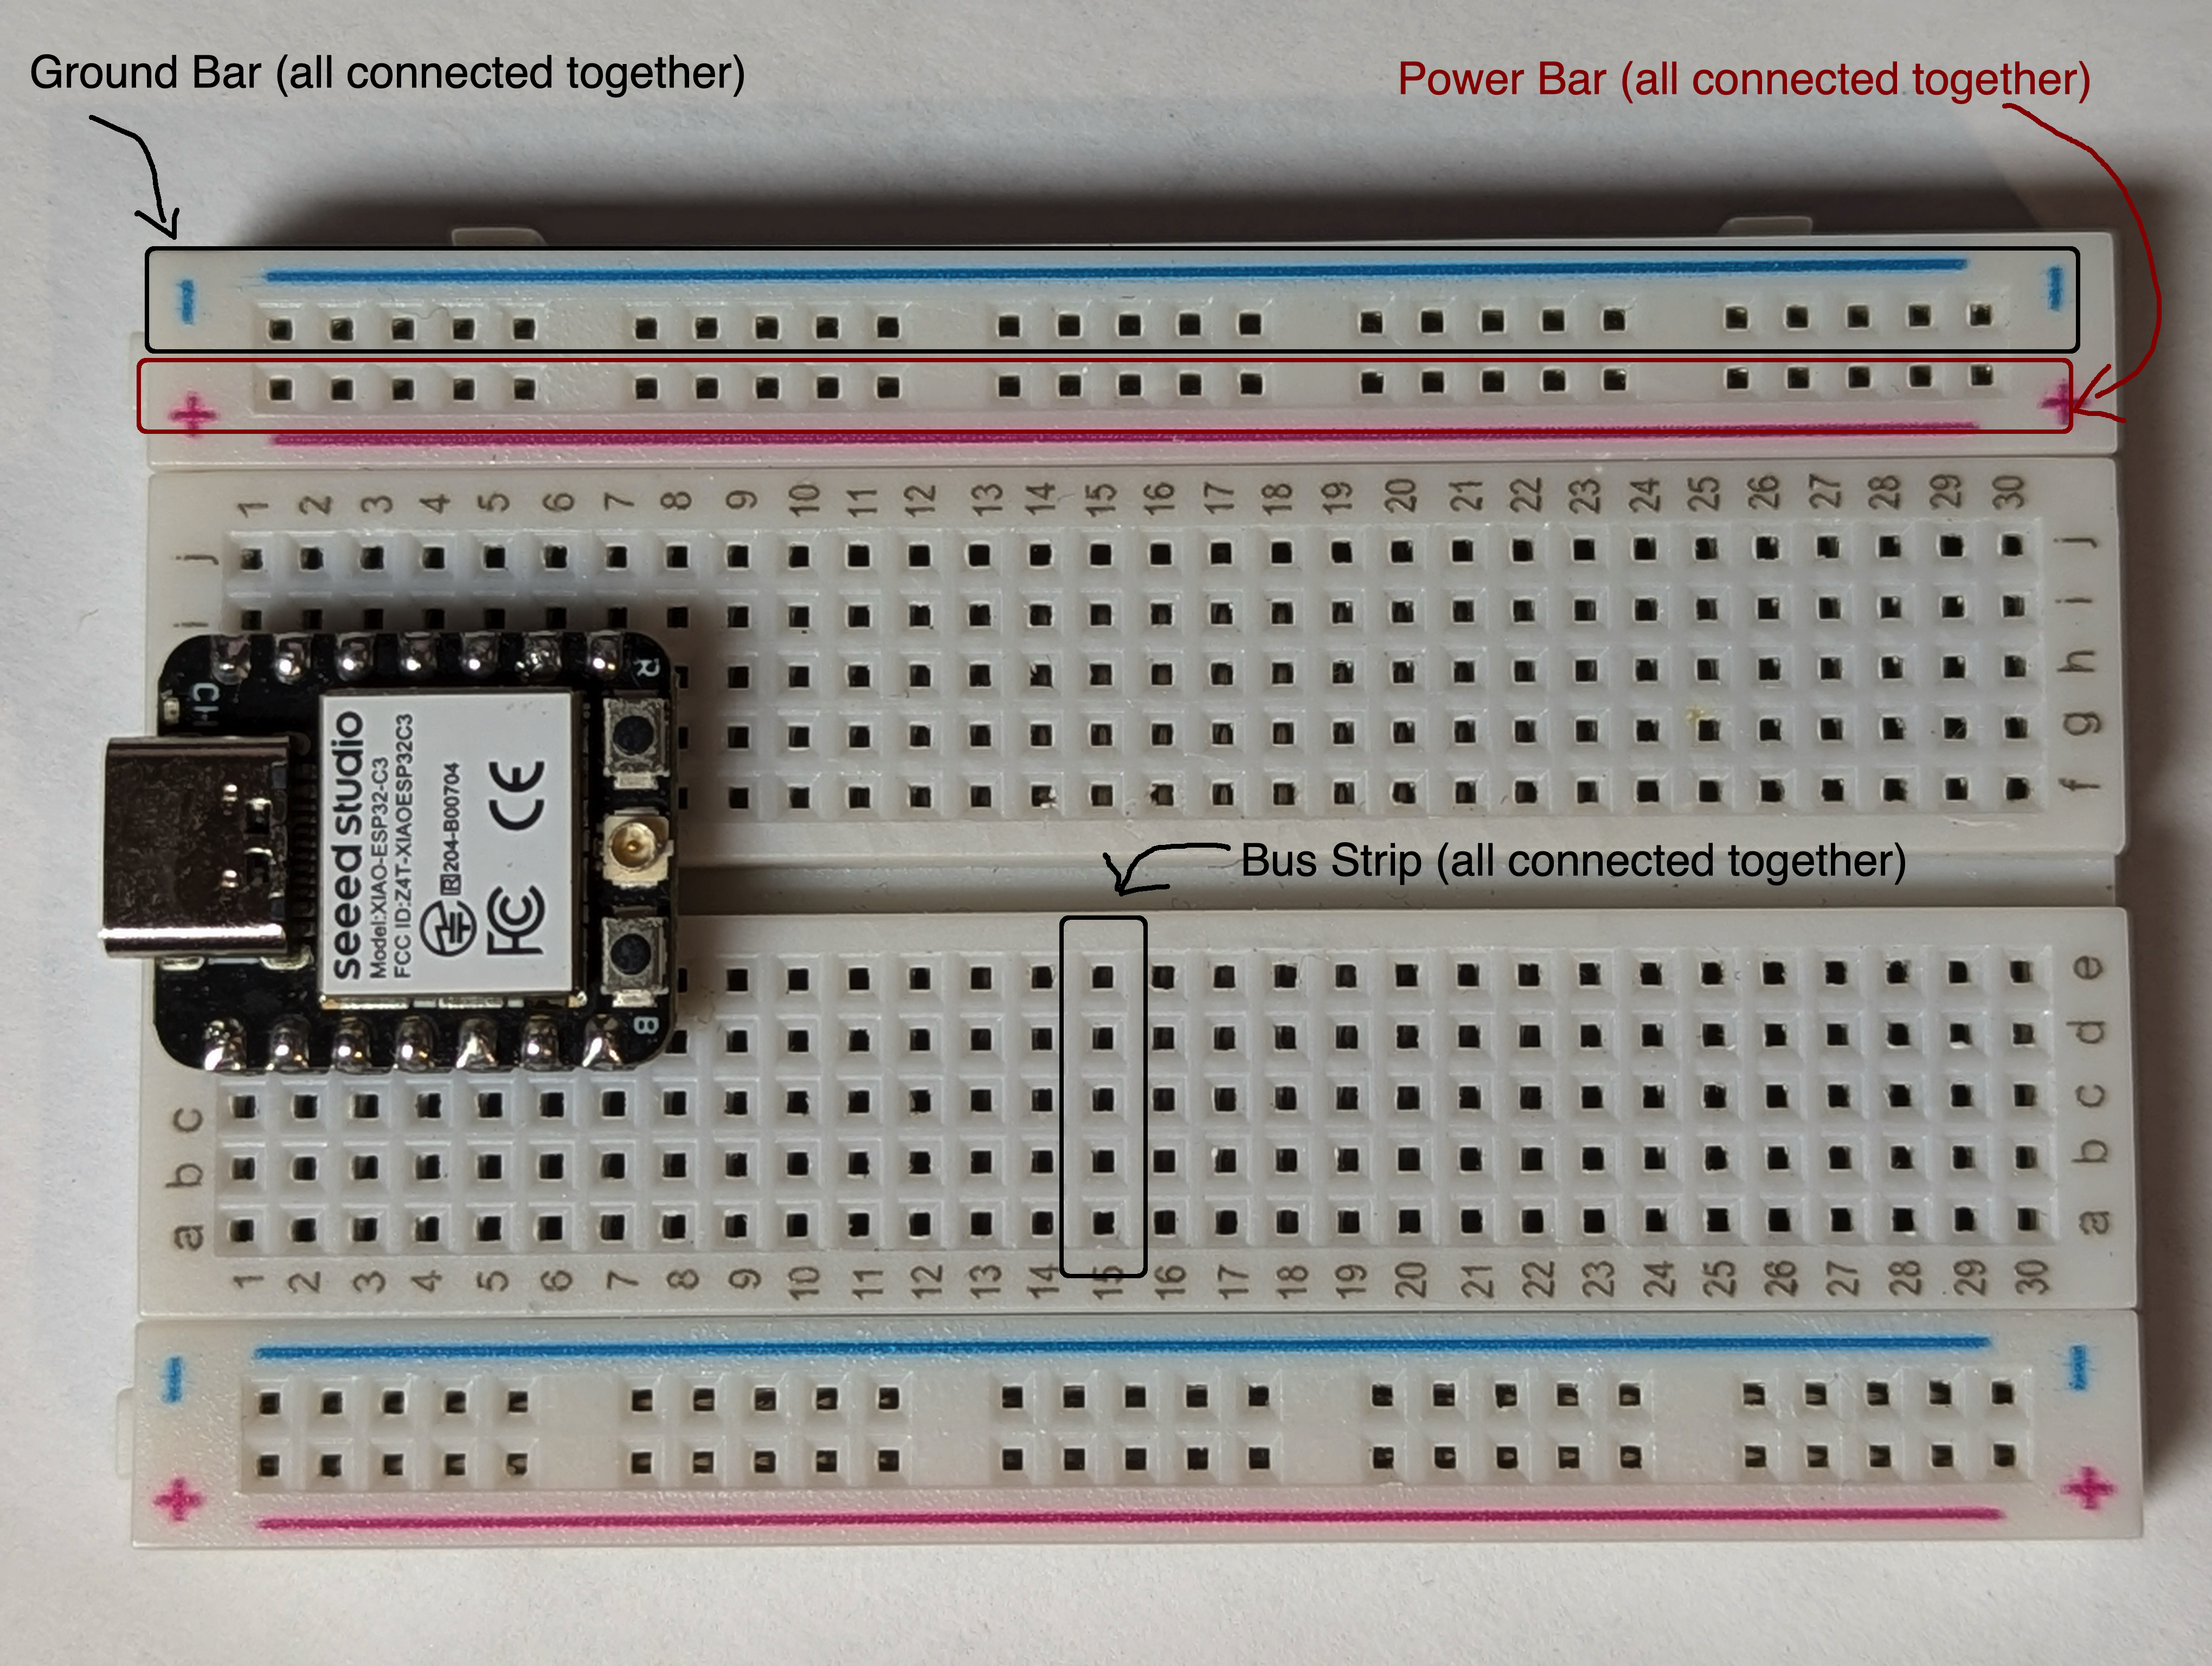
\includegraphics[width=.8\linewidth]{electronics_preamble/breadboard_illustration.png}
\end{figure}

\section{LEDs: Lighting Up Your Circuits}
\subsection{What is an LED?}
An LED (Light-Emitting Diode) is a semiconductor device that emits light when an electric current
passes through it. They are available in various colors and are commonly used as indicators or
displays in electronic circuits.

\subsection{Polarity}
LEDs have two leads:
\begin{itemize}
\item \textbf{Anode (longer lead):} Connected to the positive (+) side of the power supply.
\item \textbf{Cathode (shorter lead):} Connected to the negative (-) side of the power supply.
\end{itemize}

\begin{figure}[H]
\centering
    \includegraphics[width=.8\linewidth]{electronics_preamble/led_illustration.png}
\end{figure}

\subsection{Current limiting resistor}
It's crucial to connect a resistor in series with an LED to limit the current flowing through it.
Otherwise, the LED may get damaged or burn out. The value of the resistor depends on the LED's
specifications and the power supply voltage.

\section{Buttons: Interacting with Your Circuits} \label{button_basics}
\subsection{What is a button?}
A button, also known as a pushbutton switch, is a simple mechanical device that completes or breaks
an electrical circuit when pressed. They are commonly used to trigger actions or provide input to
electronic circuits.

\subsection{Types of buttons}
\begin{itemize}
    \item \textbf{Normally open (NO):} The circuit is open (no connection) when the button is not
    pressed and closes (connection made) when pressed.
    \item \textbf{Normally closed (NC):} The circuit is closed (connection made) when the button is
    not pressed and opens (no connection) when pressed.
\end{itemize}

\subsection{Connected Pins}
Many buttons will have more than two pins (often 4). If they do, then often you can see on the bottom
that some of those pins will already be connected together. Pay attention to this so that you wire it
up the right way.

\begin{figure}[H]
\centering
    \includegraphics[width=.8\linewidth]{electronics_preamble/button_illustration.png}
\end{figure}

\section{Jumper Cables: Making Connections}
\subsection{What are jumper cables?}
Jumper cables are short wires with connectors at both ends used to make temporary connections between
components on a breadboard or between a breadboard and other devices.

\subsection{Using jumper cables}
Insert the connectors into the appropriate holes on the breadboard or device to establish a connection.

\begin{figure}[H]
\centering
    \includegraphics[width=.7\linewidth]{electronics_preamble/jumper_illustration.png}
\end{figure}

\section{Resistors: Controlling Current Flow}
\subsection{What is a resistor?}
A resistor is a passive component that limits the flow of electric current in a circuit. They are
essential for protecting components (like LEDs) from excessive current and for controlling voltage
levels in circuits.

\subsection{Resistance value}
The resistance value is measured in ohms (\si{\ohm}) and is indicated by colored bands on the resistor body.
You can use a resistor color code chart to decode the value.

\begin{figure}[H]
\centering
    \includegraphics[width=.8\linewidth]{electronics_preamble/resistor_illustration.png}
\end{figure}

\section{Safety Tips:}
\begin{itemize}
    \item Always disconnect the power supply before making any changes to the circuit.
    \item Be careful not to short-circuit the power supply by connecting the positive and negative rails directly.
    \item If you smell burning or see smoke, immediately disconnect the power supply.
\end{itemize}
